% Options for packages loaded elsewhere
\PassOptionsToPackage{unicode}{hyperref}
\PassOptionsToPackage{hyphens}{url}
\PassOptionsToPackage{dvipsnames,svgnames,x11names}{xcolor}
%
\documentclass[
  article]{jss}

\usepackage{amsmath,amssymb}
\usepackage{iftex}
\ifPDFTeX
  \usepackage[T1]{fontenc}
  \usepackage[utf8]{inputenc}
  \usepackage{textcomp} % provide euro and other symbols
\else % if luatex or xetex
  \usepackage{unicode-math}
  \defaultfontfeatures{Scale=MatchLowercase}
  \defaultfontfeatures[\rmfamily]{Ligatures=TeX,Scale=1}
\fi
\usepackage{lmodern}
\ifPDFTeX\else  
    % xetex/luatex font selection
\fi
% Use upquote if available, for straight quotes in verbatim environments
\IfFileExists{upquote.sty}{\usepackage{upquote}}{}
\IfFileExists{microtype.sty}{% use microtype if available
  \usepackage[]{microtype}
  \UseMicrotypeSet[protrusion]{basicmath} % disable protrusion for tt fonts
}{}
\makeatletter
\@ifundefined{KOMAClassName}{% if non-KOMA class
  \IfFileExists{parskip.sty}{%
    \usepackage{parskip}
  }{% else
    \setlength{\parindent}{0pt}
    \setlength{\parskip}{6pt plus 2pt minus 1pt}}
}{% if KOMA class
  \KOMAoptions{parskip=half}}
\makeatother
\usepackage{xcolor}
\setlength{\emergencystretch}{3em} % prevent overfull lines
\setcounter{secnumdepth}{-\maxdimen} % remove section numbering
% Make \paragraph and \subparagraph free-standing
\ifx\paragraph\undefined\else
  \let\oldparagraph\paragraph
  \renewcommand{\paragraph}[1]{\oldparagraph{#1}\mbox{}}
\fi
\ifx\subparagraph\undefined\else
  \let\oldsubparagraph\subparagraph
  \renewcommand{\subparagraph}[1]{\oldsubparagraph{#1}\mbox{}}
\fi


\providecommand{\tightlist}{%
  \setlength{\itemsep}{0pt}\setlength{\parskip}{0pt}}\usepackage{longtable,booktabs,array}
\usepackage{calc} % for calculating minipage widths
% Correct order of tables after \paragraph or \subparagraph
\usepackage{etoolbox}
\makeatletter
\patchcmd\longtable{\par}{\if@noskipsec\mbox{}\fi\par}{}{}
\makeatother
% Allow footnotes in longtable head/foot
\IfFileExists{footnotehyper.sty}{\usepackage{footnotehyper}}{\usepackage{footnote}}
\makesavenoteenv{longtable}
\usepackage{graphicx}
\makeatletter
\def\maxwidth{\ifdim\Gin@nat@width>\linewidth\linewidth\else\Gin@nat@width\fi}
\def\maxheight{\ifdim\Gin@nat@height>\textheight\textheight\else\Gin@nat@height\fi}
\makeatother
% Scale images if necessary, so that they will not overflow the page
% margins by default, and it is still possible to overwrite the defaults
% using explicit options in \includegraphics[width, height, ...]{}
\setkeys{Gin}{width=\maxwidth,height=\maxheight,keepaspectratio}
% Set default figure placement to htbp
\makeatletter
\def\fps@figure{htbp}
\makeatother

\usepackage{orcidlink,thumbpdf,lmodern}

\newcommand{\class}[1]{`\code{#1}'}
\newcommand{\fct}[1]{\code{#1()}}
\makeatletter
\makeatother
\makeatletter
\makeatother
\makeatletter
\@ifpackageloaded{caption}{}{\usepackage{caption}}
\AtBeginDocument{%
\ifdefined\contentsname
  \renewcommand*\contentsname{Table of contents}
\else
  \newcommand\contentsname{Table of contents}
\fi
\ifdefined\listfigurename
  \renewcommand*\listfigurename{List of Figures}
\else
  \newcommand\listfigurename{List of Figures}
\fi
\ifdefined\listtablename
  \renewcommand*\listtablename{List of Tables}
\else
  \newcommand\listtablename{List of Tables}
\fi
\ifdefined\figurename
  \renewcommand*\figurename{Figure}
\else
  \newcommand\figurename{Figure}
\fi
\ifdefined\tablename
  \renewcommand*\tablename{Table}
\else
  \newcommand\tablename{Table}
\fi
}
\@ifpackageloaded{float}{}{\usepackage{float}}
\floatstyle{ruled}
\@ifundefined{c@chapter}{\newfloat{codelisting}{h}{lop}}{\newfloat{codelisting}{h}{lop}[chapter]}
\floatname{codelisting}{Listing}
\newcommand*\listoflistings{\listof{codelisting}{List of Listings}}
\makeatother
\makeatletter
\@ifpackageloaded{caption}{}{\usepackage{caption}}
\@ifpackageloaded{subcaption}{}{\usepackage{subcaption}}
\makeatother
\makeatletter
\makeatother
\ifLuaTeX
  \usepackage{selnolig}  % disable illegal ligatures
\fi
\IfFileExists{bookmark.sty}{\usepackage{bookmark}}{\usepackage{hyperref}}
\IfFileExists{xurl.sty}{\usepackage{xurl}}{} % add URL line breaks if available
\urlstyle{same} % disable monospaced font for URLs
\hypersetup{
  pdftitle={Team 15 The Scientists: Crime Prediction Proposal},
  pdfauthor={Xiangyu Jin (xjin13); Vinayak Bagdi (vbagdi2)},
  pdfkeywords={R, group project},
  colorlinks=true,
  linkcolor={blue},
  filecolor={Maroon},
  citecolor={Blue},
  urlcolor={Blue},
  pdfcreator={LaTeX via pandoc}}

%% -- Article metainformation (author, title, ...) -----------------------------

%% Author information
\author{Xiangyu Jin (xjin13)\\UIUC \And Vinayak Bagdi (vbagdi2)\\UIUC}
\Plainauthor{Xiangyu Jin (xjin13), Vinayak Bagdi
(vbagdi2)} %% comma-separated

\title{Team 15 The Scientists: Crime Prediction Proposal}
\Plaintitle{Team 15 The Scientists: Crime Prediction
Proposal} %% without formatting

%% an abstract and keywords
\Abstract{The project aims to predict the type of crime an arrestee may
have committed based on their background information such as race, sex,
age, and other attributes. The central idea is to examine whether there
are any relationships between crime types and arrestee's background
information and to study the crime distribution in Champaign The project
employs classification models or random forests model to predict the
crime type based on the information about the arrestees. The project
uses data before 2018 as training data and data after 2018 as testing
data to test the model's accuracy. The methods employed so far include
data cleaning, feature engineering, data manipulation, data
visualization, and data analysis using R. The implications of the work
done so far will help to improve the understanding of crime distribution
in Champaign and aid in the development of effective crime prevention
and control strategies.}

%% at least one keyword must be supplied
\Keywords{R, group project}
\Plainkeywords{R, group project}

%% publication information
%% NOTE: Typically, this can be left commented and will be filled out by the technical editor
%% \Volume{50}
%% \Issue{9}
%% \Month{June}
%% \Year{2012}
%% \Submitdate{2012-06-04}
%% \Acceptdate{2012-06-04}
%% \setcounter{page}{1}
%% \Pages{1--xx}

%% The address of (at least) one author should be given
%% in the following format:
\Address{
Xiangyu Jin (xjin13)\\
Department of Statistics\\
E-mail: \email{xjin13@illinois.edu}\\
\\~
Vinayak Bagdi (vbagdi2)\\
Department of Statistics\\
E-mail: \email{vbagdi2@illinois.edu}\\
\\~

}

\begin{document}
\maketitle
\begin{verbatim}
library(tidyverse)
\end{verbatim}

\begin{verbatim}
-- Attaching packages --------------------------------------- tidyverse 1.3.2 --
v ggplot2 3.4.1     v purrr   0.3.4
v tibble  3.1.8     v dplyr   1.0.9
v tidyr   1.2.0     v stringr 1.4.1
v readr   2.1.2     v forcats 0.5.2
-- Conflicts ------------------------------------------ tidyverse_conflicts() --
x dplyr::filter() masks stats::filter()
x dplyr::lag()    masks stats::lag()
\end{verbatim}

\begin{verbatim}
library(ggplot2)
library(hrbrthemes)
\end{verbatim}

\begin{verbatim}
NOTE: Either Arial Narrow or Roboto Condensed fonts are required to use these themes.
      Please use hrbrthemes::import_roboto_condensed() to install Roboto Condensed and
      if Arial Narrow is not on your system, please see https://bit.ly/arialnarrow
\end{verbatim}

\begin{verbatim}
library(caret)
\end{verbatim}

\begin{verbatim}
Loading required package: lattice

Attaching package: 'caret'

The following object is masked from 'package:purrr':

    lift
\end{verbatim}

\begin{verbatim}
library(ranger)
library(randomForest)
\end{verbatim}

\begin{verbatim}
randomForest 4.7-1.1
Type rfNews() to see new features/changes/bug fixes.

Attaching package: 'randomForest'

The following object is masked from 'package:ranger':

    importance

The following object is masked from 'package:dplyr':

    combine

The following object is masked from 'package:ggplot2':

    margin
\end{verbatim}

\begin{verbatim}
library(ROCR)
library(myPackage)
\end{verbatim}

\hypertarget{introduction}{%
\section{Introduction}\label{introduction}}

The project aims to examine the relationship between the type of crime
and the background information of the arrestees, including race, sex,
age, and other attributes. The problem being addressed is the high rate
of crime in Champaign, which poses a significant threat to the safety
and well-being of residents. It is essential to develop effective crime
prevention and control strategies that take into account the underlying
factors contributing to crime. The objective of the project is to
predict the type of crime an arrestee may have committed based on their
background information, which can aid in developing effective crime
prevention strategies.

The motivation for pursuing this problem is to improve the understanding
of crime distribution in Champaign and to identify potential factors
contributing to the high rate of crime. The project can aid in the
development of targeted crime prevention and control strategies that can
help to reduce crime rates in the city. Additionally, the project can
help law enforcement agencies to allocate resources effectively and
efficiently.

\hypertarget{related-works}{%
\section{Related Works}\label{related-works}}

\citet{Travaini2022} explores the use of machine learning algorithms to
predict the likelihood of criminal recidivism. The study used a dataset
consisting of demographic and criminal history variables of inmates to
develop a prediction model. This study is relevant to our project as it
also uses machine learning algorithms to predict criminal activities
based on input features. However, the focus of our project is on
predicting the type of crime based on the background information of the
arrestees, whereas the study by \citet{Travaini2022} is focused on
predicting the likelihood of criminal recidivism. Both employ machine
learning algorithms to predict criminal activities based on input
features. However, the input features and prediction targets are
different. Our project focuses on predicting the type of crime based on
the background information of the arrestees, whereas the study by
\citet{Travaini2022} focuses on predicting the likelihood of criminal
recidivism based on demographic and criminal history variables of
inmates.

\citet{Saeed2015} explores the use of machine learning algorithms to
classify criminal activities based on the input features. The study used
a dataset consisting of demographic and behavioral variables of
criminals to develop a prediction model.This study is relevant to the
current project as it also uses machine learning algorithms to predict
criminal activities based on input features. The focus of our project is
on predicting the type of crime based on the background information of
the arrestees, whereas the study by \citet{Saeed2015} is focused on
classifying criminal activities based on the input features. Both employ
machine learning algorithms to predict criminal activities based on
input features. However, the prediction targets are different. Our
project focuses on predicting the type of crime based on the background
information of the arrestees, whereas the study by \citet{Saeed2015}
focuses on classifying criminal activities based on the input features.

\citet{Mandalapu2023} is a systematic review of crime prediction using
machine learning techniques. The authors reviewed and analyzed 82
research papers from 2010 to 2019. The review highlights the importance
of data preprocessing, feature selection, and algorithm selection in
crime prediction. The authors also discuss the limitations and
challenges of using machine learning in crime prediction, such as data
imbalance, interpretability, and ethical concerns. This work relates to
our current project as it provides insights into the state of the art in
crime prediction using machine learning techniques. It highlights the
importance of data preprocessing and algorithm selection, which are
critical steps in our project. It also discusses the challenges and
limitations of using machine learning in crime prediction, which we
should be aware of when interpreting our results. Our approach will be
similar to the reviewed papers in terms of using machine learning
techniques for crime prediction. However, we will focus on a specific
dataset from Champaign and investigate the relationship between crime
types and arrestee's background information. We will also perform data
preprocessing, feature engineering, and model selection based on the
characteristics of our dataset.

\citet{Pearsall2016} analyzes the implementation and impact of
predictive policing practices in Baltimore, Maryland. The authors use
administrative data from the Baltimore Police Department to evaluate the
accuracy and effectiveness of crime predictions and to examine the
potential biases and ethical implications of using predictive policing.
The study finds that predictive policing does not significantly reduce
crime and may exacerbate existing racial and socioeconomic disparities
in policing. This work relates to our project as it raises important
ethical and social issues in crime prediction using machine learning. It
highlights the potential biases and unintended consequences of using
predictive policing and emphasizes the need for transparency and
accountability in policing practices. Our approach will differ from the
reviewed paper as we will not be directly implementing predictive
policing. However, we will be using models to predict crime types based
on arrestee's background information, which raises similar ethical and
social concerns. We will need to consider the potential biases and
unintended consequences of using our models and ensure that our results
are transparent and accountable.

\citet{Lin2018} proposes a crime prediction model based on long
short-term memory (LSTM) neural networks. The authors use crime data
from a police department in China to train and test their model. They
compare the performance of their LSTM model with other machine learning
models and find that LSTM outperforms traditional models in predicting
crime. This work relates to our project as it proposes a machine
learning model specifically designed for crime prediction. It suggests
that deep learning models, such as LSTM, may be more suitable for
capturing the temporal patterns and dependencies in crime data. We can
consider using LSTM or other deep learning models as an alternative
approach to our prediction task. Our approach will be similar to the
reviewed paper in terms of using machine learning models for crime
prediction. However, we will be using a different dataset from Champaign
and a different set of predictors. We will also be comparing the
performance of different machine learning models to select the best
model for our task. \#\# Data

\begin{verbatim}
# Reading online CSV file with big limit
my_data = load_data()
\end{verbatim}

\begin{verbatim}
Warning: One or more parsing issues, see `problems()` for details
\end{verbatim}

\begin{verbatim}
Rows: 216554 Columns: 25
-- Column specification --------------------------------------------------------
Delimiter: ","
chr  (19): arrest_code, incident_number, arrest_type_description, crime_code...
dbl   (4): year_of_arrest, month_of_arrest, disposition_code, age_at_arrest
lgl   (1): conspiracy_code
dttm  (1): date_of_arrest

i Use `spec()` to retrieve the full column specification for this data.
i Specify the column types or set `show_col_types = FALSE` to quiet this message.
\end{verbatim}

\begin{verbatim}
summary(my_data)
\end{verbatim}

\begin{verbatim}
 arrest_code        incident_number    date_of_arrest                 
 Length:216554      Length:216554      Min.   :1988-01-01 00:00:00.0  
 Class :character   Class :character   1st Qu.:1996-07-10 00:00:00.0  
 Mode  :character   Mode  :character   Median :2004-07-05 00:00:00.0  
                                       Mean   :2004-08-27 15:07:28.5  
                                       3rd Qu.:2012-06-21 00:00:00.0  
                                       Max.   :2023-02-14 00:00:00.0  
                                       NA's   :1                      
 year_of_arrest month_of_arrest  arrest_type_description  crime_code       
 Min.   :1988   Min.   : 1.000   Length:216554           Length:216554     
 1st Qu.:1996   1st Qu.: 4.000   Class :character        Class :character  
 Median :2004   Median : 6.000   Mode  :character        Mode  :character  
 Mean   :2004   Mean   : 6.458                                             
 3rd Qu.:2012   3rd Qu.: 9.000                                             
 Max.   :2023   Max.   :12.000                                             
 NA's   :1      NA's   :1                                                  
 crime_code_description crime_category_code crime_category_description
 Length:216554          Length:216554       Length:216554             
 Class :character       Class :character    Class :character          
 Mode  :character       Mode  :character    Mode  :character          
                                                                      
                                                                      
                                                                      
                                                                      
 conspiracy_code   statute           violation         disposition_code
 Mode:logical    Length:216554      Length:216554      Min.   :86.00   
 TRUE:2          Class :character   Class :character   1st Qu.:87.00   
 NA's:216552     Mode  :character   Mode  :character   Median :87.00   
                                                       Mean   :87.81   
                                                       3rd Qu.:88.00   
                                                       Max.   :98.00   
                                                       NA's   :1       
 disposition_description age_at_arrest      arrestee_sex      
 Length:216554           Min.   :-7172.00   Length:216554     
 Class :character        1st Qu.:   20.00   Class :character  
 Mode  :character        Median :   26.00   Mode  :character  
                         Mean   :   29.48                     
                         3rd Qu.:   36.00                     
                         Max.   :   99.00                     
                         NA's   :1                            
 arrestee_race      arrestee_employment_description
 Length:216554      Length:216554                  
 Class :character   Class :character               
 Mode  :character   Mode  :character               
                                                   
                                                   
                                                   
                                                   
 arrestee_residency_description arrestee_home_city arrestee_home_state
 Length:216554                  Length:216554      Length:216554      
 Class :character               Class :character   Class :character   
 Mode  :character               Mode  :character   Mode  :character   
                                                                      
                                                                      
                                                                      
                                                                      
 arrestee_home_zip  arrest_resolution  mapped_address    
 Length:216554      Length:216554      Length:216554     
 Class :character   Class :character   Class :character  
 Mode  :character   Mode  :character   Mode  :character  
                                                         
                                                         
                                                         
                                                         
\end{verbatim}

The data set contains both numerical and character data. City of Urbana
collected the data and this data set is available on Urbana's Open Data
website. The whole data set contains 216554 observations and 25
features. The data set is updated monthly with two months lag. The data
set is in CSV form. When we load the data, we need to specify length of
csv file as large as possible. Otherwise, only first 1000 observations
will be loaded.

\begin{verbatim}
# First five observations of the dataset. 
head(my_data, n = 5)
\end{verbatim}

\begin{verbatim}
# A tibble: 5 x 25
  arrest_c~1 incid~2 date_of_arrest      year_~3 month~4 arres~5 crime~6 crime~7
  <chr>      <chr>   <dttm>                <dbl>   <dbl> <chr>   <chr>   <chr>  
1 A23-00466  T23-00~ 2023-02-14 00:00:00    2023       2 SUMMON~ 2460    CANCEL~
2 A23-00459  T23-00~ 2023-02-13 00:00:00    2023       2 SUMMON~ 2481    DRIVIN~
3 A23-00461  U23-02~ 2023-02-13 00:00:00    2023       2 SUMMON~ 6621    FAILUR~
4 A23-00463  U23-02~ 2023-02-13 00:00:00    2023       2 SUMMON~ 6617    FAILUR~
5 A23-00465  U23-02~ 2023-02-13 00:00:00    2023       2 SUMMON~ 2461    OPERAT~
# ... with 17 more variables: crime_category_code <chr>,
#   crime_category_description <chr>, conspiracy_code <lgl>, statute <chr>,
#   violation <chr>, disposition_code <dbl>, disposition_description <chr>,
#   age_at_arrest <dbl>, arrestee_sex <chr>, arrestee_race <chr>,
#   arrestee_employment_description <chr>,
#   arrestee_residency_description <chr>, arrestee_home_city <chr>,
#   arrestee_home_state <chr>, arrestee_home_zip <chr>, ...
\end{verbatim}

\hypertarget{eda}{%
\section{EDA}\label{eda}}

\begin{verbatim}
my_data %>%
  select(where(is.numeric)) %>% 
  summary()
\end{verbatim}

\begin{verbatim}
 year_of_arrest month_of_arrest  disposition_code age_at_arrest     
 Min.   :1988   Min.   : 1.000   Min.   :86.00    Min.   :-7172.00  
 1st Qu.:1996   1st Qu.: 4.000   1st Qu.:87.00    1st Qu.:   20.00  
 Median :2004   Median : 6.000   Median :87.00    Median :   26.00  
 Mean   :2004   Mean   : 6.458   Mean   :87.81    Mean   :   29.48  
 3rd Qu.:2012   3rd Qu.: 9.000   3rd Qu.:88.00    3rd Qu.:   36.00  
 Max.   :2023   Max.   :12.000   Max.   :98.00    Max.   :   99.00  
 NA's   :1      NA's   :1        NA's   :1        NA's   :1         
\end{verbatim}

\hypertarget{data-cleaning-and-feature-engineering}{%
\subsection{Data Cleaning and Feature
Engineering}\label{data-cleaning-and-feature-engineering}}

\begin{verbatim}
my_data = myPackage::process_data(my_data)
\end{verbatim}

\begin{verbatim}
summary(my_data)
\end{verbatim}

\begin{verbatim}
 incident_number    year_of_arrest month_of_arrest  crime_category_description
 Length:112059      Min.   :2000   Min.   : 1.000   Length:112059             
 Class :character   1st Qu.:2004   1st Qu.: 4.000   Class :character          
 Mode  :character   Median :2009   Median : 6.000   Mode  :character          
                    Mean   :2009   Mean   : 6.427                             
                    3rd Qu.:2014   3rd Qu.: 9.000                             
                    Max.   :2019   Max.   :12.000                             
 age_at_arrest   arrestee_sex       arrestee_race     
 Min.   : 9.00   Length:112059      Length:112059     
 1st Qu.:21.00   Class :character   Class :character  
 Median :26.00   Mode  :character   Mode  :character  
 Mean   :30.47                                        
 3rd Qu.:37.00                                        
 Max.   :99.00                                        
 arrestee_employment_description arrestee_home_city arrestee_home_state
 Length:112059                   Length:112059      Length:112059      
 Class :character                Class :character   Class :character   
 Mode  :character                Mode  :character   Mode  :character   
                                                                       
                                                                       
                                                                       
   homecity        
 Length:112059     
 Class :character  
 Mode  :character  
                   
                   
                   
\end{verbatim}

\begin{verbatim}
sum(is.na(my_data))
\end{verbatim}

\begin{verbatim}
[1] 0
\end{verbatim}

After data cleaning and feature engineering, we filter the data only
after year 2000. Moreover, we only select variables
\texttt{incident\_number}, \texttt{year\_of\_arrest},
\texttt{month\_of\_arrest},\texttt{crime\_category\_description},
\texttt{age\_at\_arrest}, \texttt{arrestee\_sex},
\texttt{arrestee\_race}, \texttt{arrestee\_employment\_description},
\texttt{arrestee\_home\_city}, and \texttt{arrestee\_home\_state} to use
in our model. Since other variables such as \texttt{arrest\_code} do not
seem relate to crime prediction.

\hypertarget{plots}{%
\subsubsection{Plots}\label{plots}}

\begin{verbatim}
# number of cases versus time (year)
myPackage::tn_plot(my_data)
\end{verbatim}

\begin{figure}[H]

{\centering 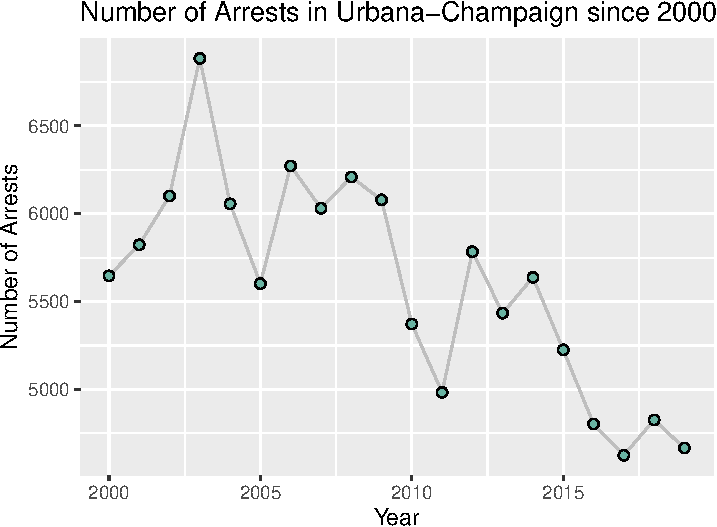
\includegraphics{final-report_files/figure-pdf/unnamed-chunk-8-1.pdf}

}

\end{figure}

Based on this graph, we can see that 2003 has the highest number of
arrests from 2000 to 2023. Moreover, there is a decreasing trend on
number of arrests through out years.

\begin{verbatim}
# Graph to see in each year arrestees sex proportion
myPackage::ts_plot(my_data)
\end{verbatim}

\begin{figure}[H]

{\centering 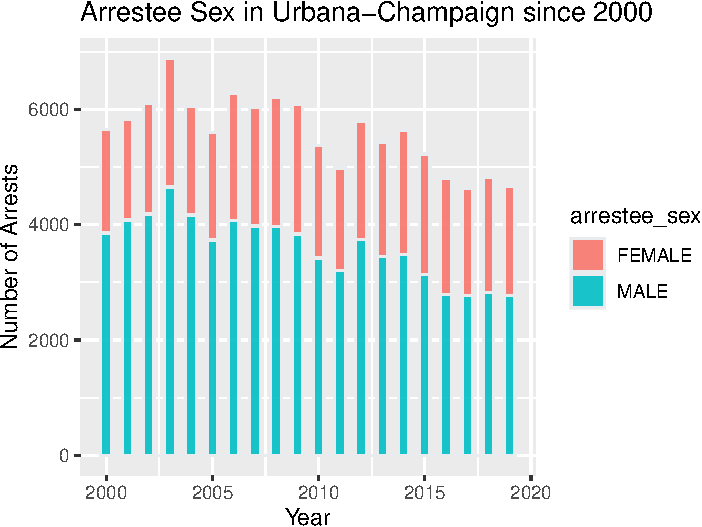
\includegraphics{final-report_files/figure-pdf/unnamed-chunk-9-1.pdf}

}

\end{figure}

Based on this graph, we can see that Male contributes over 50\% of
arrests each year, which means that MALE is more likely to got arrested
compared with FEMALE.

\begin{verbatim}
# Graph to see in each year arrestee race proportion
myPackage::tr_plot(my_data)
\end{verbatim}

\begin{figure}[H]

{\centering 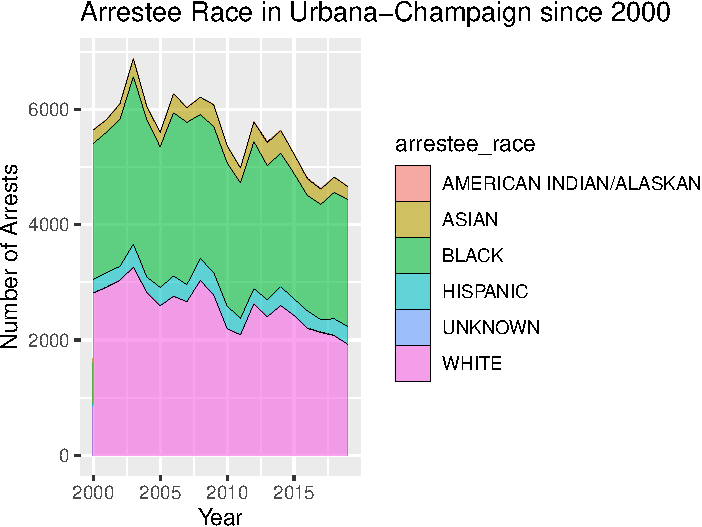
\includegraphics{final-report_files/figure-pdf/unnamed-chunk-10-1.pdf}

}

\end{figure}

Based on this graph, we can see there BALCK and WHITE contribute over
80\% arrests. We can roughly see that WHITE contributes a little more
than BLACK.

\begin{verbatim}
## Graph to show proportions of arrestee home city in each year
myPackage::th_plot(my_data)
\end{verbatim}

\begin{figure}[H]

{\centering 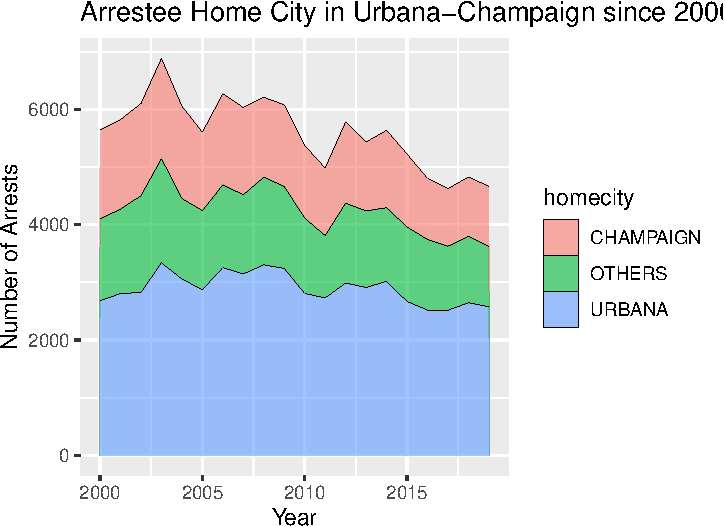
\includegraphics{final-report_files/figure-pdf/unnamed-chunk-11-1.pdf}

}

\end{figure}

Based on this graph, we can see that most arrestees are from URBANA.
Arrestess from CHAMPAIGN and Other home cities roughtly contribute the
same to the total number of arrests in each year.

\begin{verbatim}
# Create visulization to see age distribution in each year
myPackage::ta_plot(my_data)
\end{verbatim}

\begin{figure}[H]

{\centering 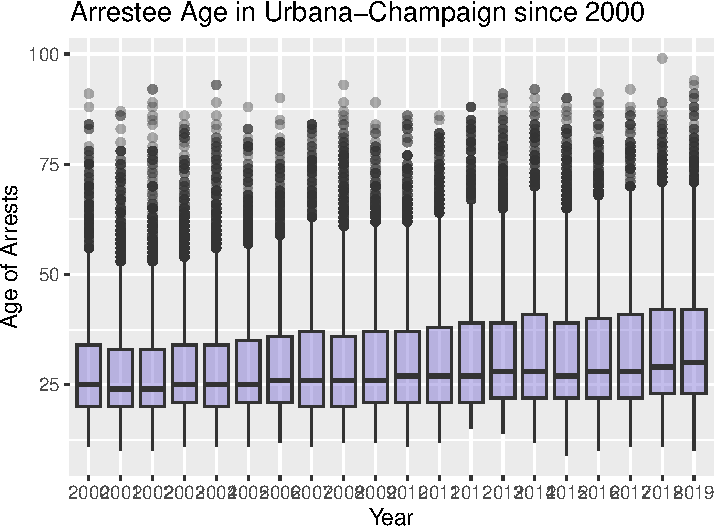
\includegraphics{final-report_files/figure-pdf/unnamed-chunk-12-1.pdf}

}

\end{figure}

As shown in the graph, we can see that the average age of arrestees in
each year is gradually increasing. And the range of age is also
increasing along the year. Age distribution seems more spread out along
th year.

\begin{verbatim}
# Create visulization to see relationship between arrestee sex and arrestee race
myPackage::sr_plot(my_data)
\end{verbatim}

\begin{figure}[H]

{\centering 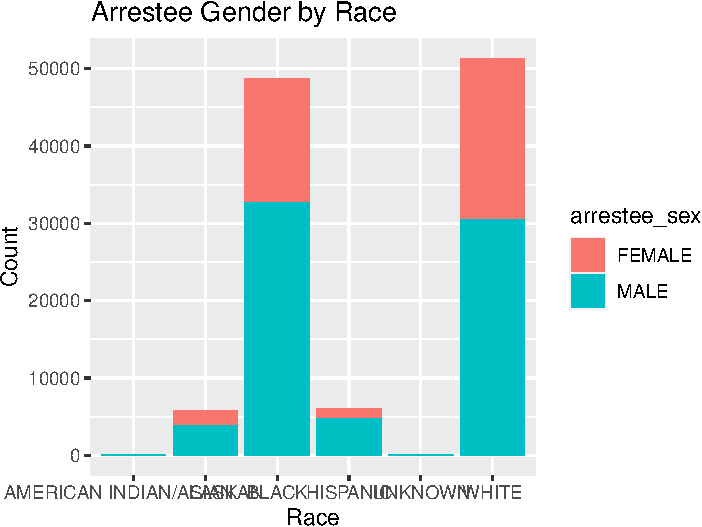
\includegraphics{final-report_files/figure-pdf/unnamed-chunk-13-1.pdf}

}

\end{figure}

In the graph above, we can see that MALE contributes more than FEMALE in
ASIAN, BLACK, HISPANIC, and WHITE races. Especially in ASIAN and
HISPANIC races, we need to consider the correlation between races and
sex. Moreover, counts of AMERICAN INDIAN?ALASKAS and UNKOWN races are so
few that we might consider drop it in modeling.

\hypertarget{method-and-results}{%
\subsection{Method and Results}\label{method-and-results}}

\hypertarget{random-forests}{%
\subsubsection{Random Forests}\label{random-forests}}

The modeling technique we are going to use is Random Forests. Random
Forests is a machine learning algorithm that combines multiple decision
trees to produce a more accurate and stable prediction. It reduces
overfitting by building each tree on a random subset of the data and a
random subset of the features. It handles both categorical and numerical
data, is less sensitive to outliers and noise, and can handle missing
data. Random Forests has many applications, including predictive
modeling in various fields, feature selection, anomaly detection, and
image and text classification. It is easy to interpret and visualize the
results, making it a powerful and popular algorithm in the machine
learning community.

We choose random forests as our modeling algorithm because Random
Forests can handle complex and non-linear relationships between the
input features and the target variable. It can capture interactions and
correlations between the variables, which may not be captured by simpler
models such as linear regression. And more importantly, it can dorectly
handle both categorical and numerical data since we have both type in
our data set.

In this algorithm, precision, which is the proportion of true positives
out of the total predicted positives, will be used to assess the model's
performance. It measures the model's ability to identify true positives

\hypertarget{results}{%
\subsubsection{Results}\label{results}}

\begin{verbatim}
# Split the data
set.seed(447)

model_data = myPackage::model_data(my_data)


rf_model = myPackage::model(model_data)

print(rf_model)
\end{verbatim}

\begin{verbatim}
Random Forest 

76048 samples
    6 predictor
   21 classes: 'Animal Offenses', 'Assault', 'Battery', 'Burglary', 'Cannabis Offenses', 'Controlled Substance Offenses', 'Criminal Damage', 'Deception & Fraud', 'Disorderly Conduct', 'Driving Under the Influence', 'Drug Paraphernalia Act', 'Interfering w/Public Officers', 'Liquor Offenses', 'Noise & Vibrations Violations', 'Offenses Involving Children', 'Prob/Parole/Bail Violations', 'Theft', 'Traffic Offenses', 'Trespassing', 'Warrants & Summons', 'Weapons Offenses' 

No pre-processing
Resampling: Cross-Validated (2 fold) 
Summary of sample sizes: 38024, 38024 
Resampling results across tuning parameters:

  mtry  Accuracy   Kappa    
   2    0.6168078  0.3006028
   8    0.6169788  0.3285411
  14    0.5762282  0.2940076

Accuracy was used to select the optimal model using the largest value.
The final value used for the model was mtry = 8.
\end{verbatim}

\begin{verbatim}
# best mtry 8
# get the test data 
set.seed(447)
trainIndex <- createDataPartition(1:nrow(model_data), p = 0.7, list = FALSE)
test <- model_data[-trainIndex, ]

prediction = predict(rf_model, test)

# evaluation
confusionMatrix(prediction, as.factor(test$crime_category_description))
\end{verbatim}

\begin{verbatim}
Confusion Matrix and Statistics

                               Reference
Prediction                      Animal Offenses Assault Battery Burglary
  Animal Offenses                            16       0      11        0
  Assault                                     0       0       5        0
  Battery                                    10      19     162       26
  Burglary                                    0       0      11        8
  Cannabis Offenses                           0       4      10        5
  Controlled Substance Offenses               0       0       0        3
  Criminal Damage                             0       1       6        1
  Deception & Fraud                           0       1       1        0
  Disorderly Conduct                          1       1      41        7
  Driving Under the Influence                 2       3      13        1
  Drug Paraphernalia Act                      0       1       1        0
  Interfering w/Public Officers               0       3      18        3
  Liquor Offenses                             2       2      59       20
  Noise & Vibrations Violations               0       0       5        4
  Offenses Involving Children                 0       0       4        0
  Prob/Parole/Bail Violations                 0       0       1        0
  Theft                                       4       9      69       12
  Traffic Offenses                          252      86     606      113
  Trespassing                                 0       0       3        0
  Warrants & Summons                         55     106     819      123
  Weapons Offenses                            0       2       1        1
                               Reference
Prediction                      Cannabis Offenses Controlled Substance Offenses
  Animal Offenses                               0                             0
  Assault                                       0                             1
  Battery                                      38                            15
  Burglary                                      6                             1
  Cannabis Offenses                            13                             4
  Controlled Substance Offenses                 1                             2
  Criminal Damage                               0                             0
  Deception & Fraud                             0                             1
  Disorderly Conduct                            4                             2
  Driving Under the Influence                   5                             0
  Drug Paraphernalia Act                        6                             1
  Interfering w/Public Officers                16                             5
  Liquor Offenses                              78                            13
  Noise & Vibrations Violations                 1                             0
  Offenses Involving Children                   0                             0
  Prob/Parole/Bail Violations                   0                             0
  Theft                                        15                             7
  Traffic Offenses                            213                           137
  Trespassing                                   0                             0
  Warrants & Summons                          293                           212
  Weapons Offenses                              2                             0
                               Reference
Prediction                      Criminal Damage Deception & Fraud
  Animal Offenses                             0                 2
  Assault                                     3                 1
  Battery                                    44                 8
  Burglary                                    0                 1
  Cannabis Offenses                           5                 3
  Controlled Substance Offenses               0                 0
  Criminal Damage                             1                 0
  Deception & Fraud                           0                 5
  Disorderly Conduct                          8                 0
  Driving Under the Influence                 4                 1
  Drug Paraphernalia Act                      1                 0
  Interfering w/Public Officers               4                 1
  Liquor Offenses                            32                13
  Noise & Vibrations Violations               2                 1
  Offenses Involving Children                 1                 0
  Prob/Parole/Bail Violations                 1                 0
  Theft                                      10                11
  Traffic Offenses                          134               116
  Trespassing                                 0                 0
  Warrants & Summons                        212                74
  Weapons Offenses                            3                 0
                               Reference
Prediction                      Disorderly Conduct Driving Under the Influence
  Animal Offenses                                3                           3
  Assault                                        1                           0
  Battery                                       62                          24
  Burglary                                       2                           0
  Cannabis Offenses                              5                           5
  Controlled Substance Offenses                  0                           2
  Criminal Damage                                3                           0
  Deception & Fraud                              0                           0
  Disorderly Conduct                            50                           0
  Driving Under the Influence                    5                          38
  Drug Paraphernalia Act                         0                           2
  Interfering w/Public Officers                  8                           3
  Liquor Offenses                               41                          43
  Noise & Vibrations Violations                  1                           2
  Offenses Involving Children                    0                           0
  Prob/Parole/Bail Violations                    1                           0
  Theft                                         22                           6
  Traffic Offenses                             251                         532
  Trespassing                                    2                           0
  Warrants & Summons                           204                         175
  Weapons Offenses                               1                           0
                               Reference
Prediction                      Drug Paraphernalia Act
  Animal Offenses                                    0
  Assault                                            1
  Battery                                           13
  Burglary                                           0
  Cannabis Offenses                                  9
  Controlled Substance Offenses                      3
  Criminal Damage                                    0
  Deception & Fraud                                  0
  Disorderly Conduct                                 2
  Driving Under the Influence                        7
  Drug Paraphernalia Act                             0
  Interfering w/Public Officers                      1
  Liquor Offenses                                   50
  Noise & Vibrations Violations                      2
  Offenses Involving Children                        1
  Prob/Parole/Bail Violations                        0
  Theft                                             12
  Traffic Offenses                                 133
  Trespassing                                        0
  Warrants & Summons                               126
  Weapons Offenses                                   0
                               Reference
Prediction                      Interfering w/Public Officers Liquor Offenses
  Animal Offenses                                           0               2
  Assault                                                   0               4
  Battery                                                  44              29
  Burglary                                                  3               5
  Cannabis Offenses                                         9              19
  Controlled Substance Offenses                             1               0
  Criminal Damage                                           0               1
  Deception & Fraud                                         1               0
  Disorderly Conduct                                        3              16
  Driving Under the Influence                               4               6
  Drug Paraphernalia Act                                    0               0
  Interfering w/Public Officers                            10              11
  Liquor Offenses                                          29             411
  Noise & Vibrations Violations                             1               4
  Offenses Involving Children                               1               0
  Prob/Parole/Bail Violations                               1               0
  Theft                                                    19              17
  Traffic Offenses                                        348             523
  Trespassing                                               0               1
  Warrants & Summons                                      374             154
  Weapons Offenses                                          1               1
                               Reference
Prediction                      Noise & Vibrations Violations
  Animal Offenses                                           3
  Assault                                                   0
  Battery                                                  17
  Burglary                                                  1
  Cannabis Offenses                                         2
  Controlled Substance Offenses                             1
  Criminal Damage                                           1
  Deception & Fraud                                         0
  Disorderly Conduct                                        3
  Driving Under the Influence                               5
  Drug Paraphernalia Act                                    1
  Interfering w/Public Officers                             1
  Liquor Offenses                                          19
  Noise & Vibrations Violations                             4
  Offenses Involving Children                               0
  Prob/Parole/Bail Violations                               0
  Theft                                                    10
  Traffic Offenses                                        152
  Trespassing                                               0
  Warrants & Summons                                      102
  Weapons Offenses                                          0
                               Reference
Prediction                      Offenses Involving Children
  Animal Offenses                                         1
  Assault                                                 0
  Battery                                                30
  Burglary                                                1
  Cannabis Offenses                                       0
  Controlled Substance Offenses                           0
  Criminal Damage                                         0
  Deception & Fraud                                       0
  Disorderly Conduct                                      0
  Driving Under the Influence                             3
  Drug Paraphernalia Act                                  0
  Interfering w/Public Officers                           0
  Liquor Offenses                                         3
  Noise & Vibrations Violations                           0
  Offenses Involving Children                             1
  Prob/Parole/Bail Violations                             0
  Theft                                                   1
  Traffic Offenses                                       52
  Trespassing                                             0
  Warrants & Summons                                     72
  Weapons Offenses                                        1
                               Reference
Prediction                      Prob/Parole/Bail Violations Theft
  Animal Offenses                                         0     3
  Assault                                                 0     2
  Battery                                                 8    81
  Burglary                                                0    11
  Cannabis Offenses                                       1     8
  Controlled Substance Offenses                           0     1
  Criminal Damage                                         0     2
  Deception & Fraud                                       0     5
  Disorderly Conduct                                      0    14
  Driving Under the Influence                             0    13
  Drug Paraphernalia Act                                  0     4
  Interfering w/Public Officers                           0    13
  Liquor Offenses                                         2    65
  Noise & Vibrations Violations                           0     3
  Offenses Involving Children                             0     0
  Prob/Parole/Bail Violations                             0     0
  Theft                                                   3    91
  Traffic Offenses                                       45   347
  Trespassing                                             0     2
  Warrants & Summons                                     95   553
  Weapons Offenses                                        0     0
                               Reference
Prediction                      Traffic Offenses Trespassing Warrants & Summons
  Animal Offenses                              3           0                 10
  Assault                                      1           0                  0
  Battery                                     68          27                139
  Burglary                                     3           3                  7
  Cannabis Offenses                           18           1                 16
  Controlled Substance Offenses                2           0                  1
  Criminal Damage                              1           0                  1
  Deception & Fraud                            2           1                  2
  Disorderly Conduct                          22          11                 11
  Driving Under the Influence                 68           2                 12
  Drug Paraphernalia Act                       3           2                  1
  Interfering w/Public Officers               25           3                 11
  Liquor Offenses                             73          25                 53
  Noise & Vibrations Violations                1           0                  3
  Offenses Involving Children                  0           0                  2
  Prob/Parole/Bail Violations                  2           0                  1
  Theft                                       31          14                 60
  Traffic Offenses                         18020         125                861
  Trespassing                                  0           1                  1
  Warrants & Summons                         650         213               1472
  Weapons Offenses                             3           0                  1
                               Reference
Prediction                      Weapons Offenses
  Animal Offenses                              0
  Assault                                      1
  Battery                                      6
  Burglary                                     0
  Cannabis Offenses                            5
  Controlled Substance Offenses                0
  Criminal Damage                              0
  Deception & Fraud                            0
  Disorderly Conduct                           3
  Driving Under the Influence                  0
  Drug Paraphernalia Act                       0
  Interfering w/Public Officers                5
  Liquor Offenses                              6
  Noise & Vibrations Violations                0
  Offenses Involving Children                  0
  Prob/Parole/Bail Violations                  0
  Theft                                        3
  Traffic Offenses                            56
  Trespassing                                  0
  Warrants & Summons                          97
  Weapons Offenses                             1

Overall Statistics
                                          
               Accuracy : 0.6231          
                 95% CI : (0.6178, 0.6284)
    No Information Rate : 0.5829          
    P-Value [Acc > NIR] : < 2.2e-16       
                                          
                  Kappa : 0.3359          
                                          
 Mcnemar's Test P-Value : NA              

Statistics by Class:

                     Class: Animal Offenses Class: Assault Class: Battery
Sensitivity                        0.046784      0.0000000       0.087757
Specificity                        0.998729      0.9993818       0.976970
Pos Pred Value                     0.280702      0.0000000       0.186207
Neg Pred Value                     0.989979      0.9926922       0.946907
Prevalence                         0.010495      0.0073033       0.056647
Detection Rate                     0.000491      0.0000000       0.004971
Detection Prevalence               0.001749      0.0006137       0.026697
Balanced Accuracy                  0.522756      0.4996909       0.532363
                     Class: Burglary Class: Cannabis Offenses
Sensitivity                0.0244648                0.0188133
Specificity                0.9982952                0.9959557
Pos Pred Value             0.1269841                0.0915493
Neg Pred Value             0.9901922                0.9791037
Prevalence                 0.0100344                0.0212041
Detection Rate             0.0002455                0.0003989
Detection Prevalence       0.0019332                0.0043574
Balanced Accuracy          0.5113800                0.5073845
                     Class: Controlled Substance Offenses
Sensitivity                                     4.988e-03
Specificity                                     9.995e-01
Pos Pred Value                                  1.176e-01
Neg Pred Value                                  9.877e-01
Prevalence                                      1.231e-02
Detection Rate                                  6.137e-05
Detection Prevalence                            5.217e-04
Balanced Accuracy                               5.023e-01
                     Class: Criminal Damage Class: Deception & Fraud
Sensitivity                       2.151e-03                0.0210970
Specificity                       9.995e-01                0.9995672
Pos Pred Value                    5.556e-02                0.2631579
Neg Pred Value                    9.858e-01                0.9928767
Prevalence                        1.427e-02                0.0072726
Detection Rate                    3.069e-05                0.0001534
Detection Prevalence              5.524e-04                0.0005830
Balanced Accuracy                 5.008e-01                0.5103321
                     Class: Disorderly Conduct
Sensitivity                           0.075529
Specificity                           0.995333
Pos Pred Value                        0.251256
Neg Pred Value                        0.981105
Prevalence                            0.020314
Detection Rate                        0.001534
Detection Prevalence                  0.006107
Balanced Accuracy                     0.535431
                     Class: Driving Under the Influence
Sensitivity                                    0.045509
Specificity                                    0.995150
Pos Pred Value                                 0.197917
Neg Pred Value                                 0.975398
Prevalence                                     0.025623
Detection Rate                                 0.001166
Detection Prevalence                           0.005892
Balanced Accuracy                              0.520330
                     Class: Drug Paraphernalia Act
Sensitivity                              0.0000000
Specificity                              0.9992863
Pos Pred Value                           0.0000000
Neg Pred Value                           0.9889452
Prevalence                               0.0110470
Detection Rate                           0.0000000
Detection Prevalence                     0.0007058
Balanced Accuracy                        0.4996432
                     Class: Interfering w/Public Officers
Sensitivity                                     0.0117786
Specificity                                     0.9958726
Pos Pred Value                                  0.0709220
Neg Pred Value                                  0.9741424
Prevalence                                      0.0260525
Detection Rate                                  0.0003069
Detection Prevalence                            0.0043267
Balanced Accuracy                               0.5038256
                     Class: Liquor Offenses
Sensitivity                         0.34136
Specificity                         0.97999
Pos Pred Value                      0.39557
Neg Pred Value                      0.97486
Prevalence                          0.03695
Detection Rate                      0.01261
Detection Prevalence                0.03188
Balanced Accuracy                   0.66068
                     Class: Noise & Vibrations Violations
Sensitivity                                     0.0124224
Specificity                                     0.9990702
Pos Pred Value                                  0.1176471
Neg Pred Value                                  0.9902316
Prevalence                                      0.0098809
Detection Rate                                  0.0001227
Detection Prevalence                            0.0010433
Balanced Accuracy                               0.5057463
                     Class: Offenses Involving Children
Sensitivity                                   6.061e-03
Specificity                                   9.997e-01
Pos Pred Value                                1.000e-01
Neg Pred Value                                9.950e-01
Prevalence                                    5.063e-03
Detection Rate                                3.069e-05
Detection Prevalence                          3.069e-04
Balanced Accuracy                             5.029e-01
                     Class: Prob/Parole/Bail Violations Class: Theft
Sensitivity                                   0.0000000     0.074713
Specificity                                   0.9997842     0.989321
Pos Pred Value                                0.0000000     0.213615
Neg Pred Value                                0.9952733     0.964959
Prevalence                                    0.0047257     0.037376
Detection Rate                                0.0000000     0.002792
Detection Prevalence                          0.0002148     0.013072
Balanced Accuracy                             0.4998921     0.532017
                     Class: Traffic Offenses Class: Trespassing
Sensitivity                           0.9486          2.336e-03
Specificity                           0.6261          9.997e-01
Pos Pred Value                        0.7800          1.000e-01
Neg Pred Value                        0.8971          9.869e-01
Prevalence                            0.5829          1.313e-02
Detection Rate                        0.5530          3.069e-05
Detection Prevalence                  0.7089          3.069e-04
Balanced Accuracy                     0.7874          5.010e-01
                     Class: Warrants & Summons Class: Weapons Offenses
Sensitivity                            0.55235               5.464e-03
Specificity                            0.84263               9.995e-01
Pos Pred Value                         0.23815               5.556e-02
Neg Pred Value                         0.95482               9.944e-01
Prevalence                             0.08178               5.616e-03
Detection Rate                         0.04517               3.069e-05
Detection Prevalence                   0.18967               5.524e-04
Balanced Accuracy                      0.69749               5.025e-01
\end{verbatim}

Our random forest model has overall accuracy of 0.6170. It's doing well
in crimes that happened a lot but the model is doing poorly on crimes
that happened few along the time.

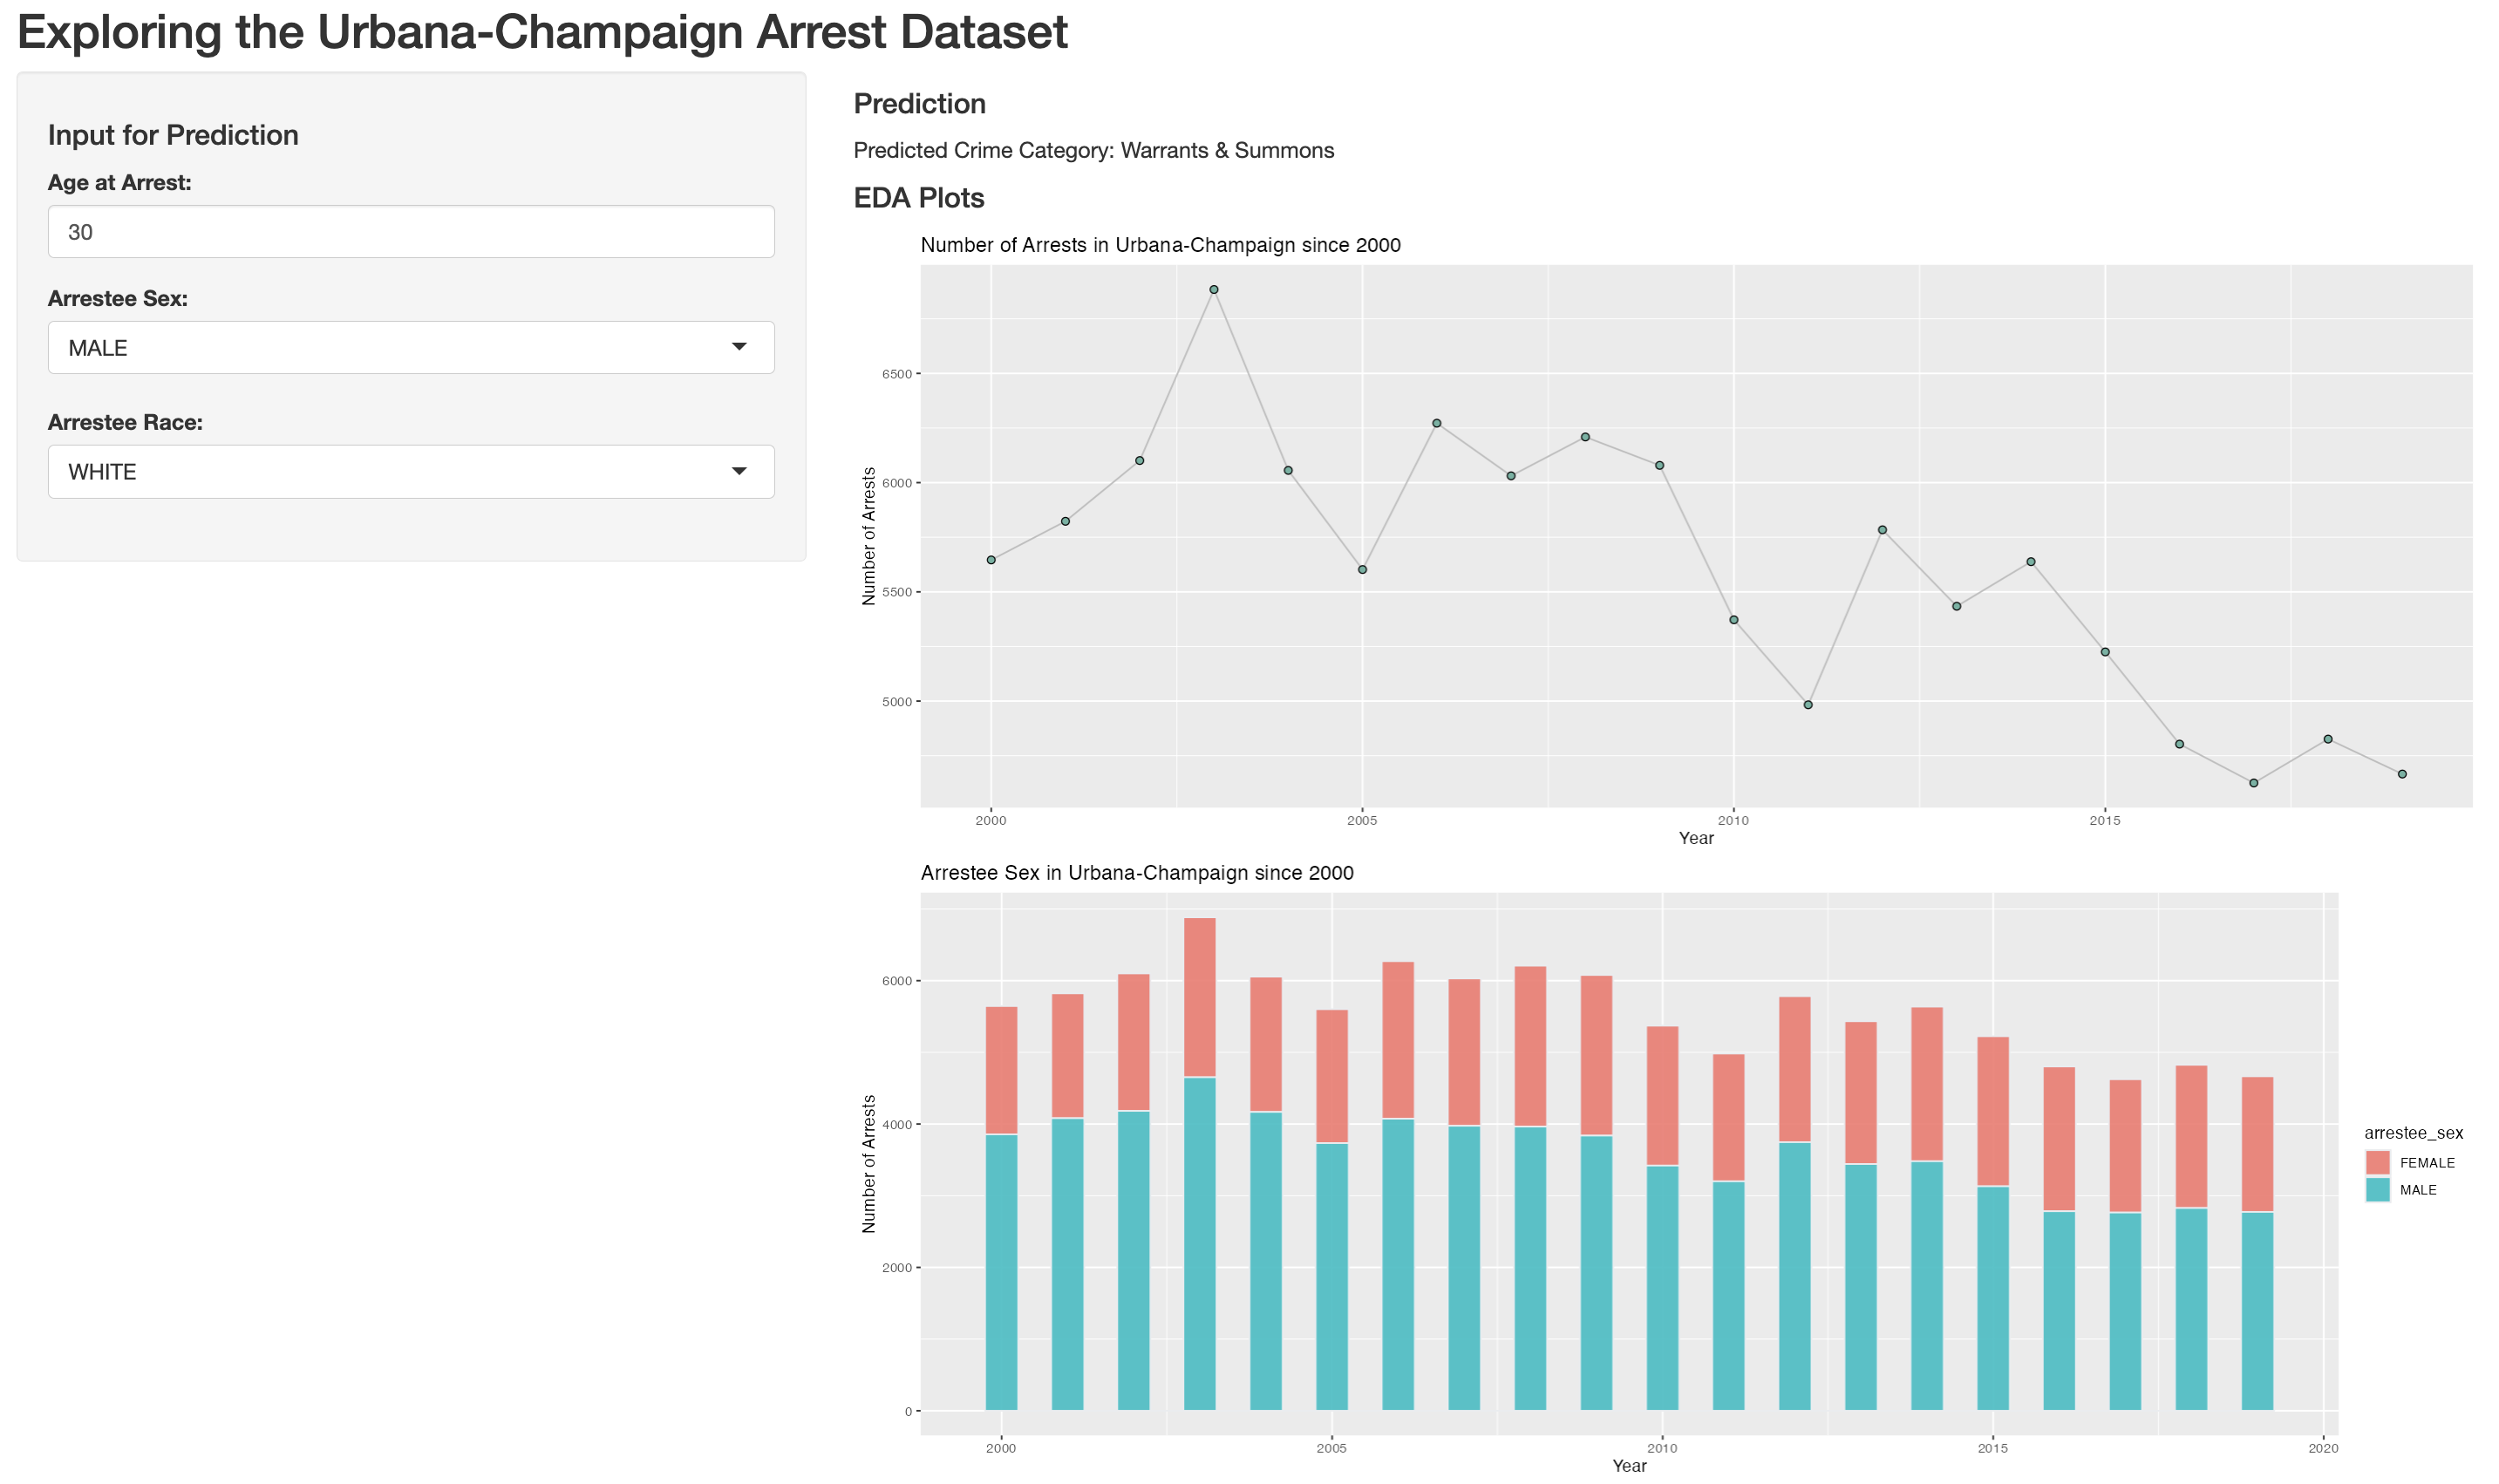
\includegraphics{shiny.png} There are three inputs in our shiny app. We
can use this shiny app to predict what type of crime the suspect is
committed to based on the inputs of suspect information. As shown in the
screenshot, our model predicts the MALE with those information inputs is
likely committed to Warrants \& Summons. It is showing the number of
arrests of different race in each year and gender proportion of
arrestees in each year. And there are six more EDA graphs below.

\hypertarget{conclusion-and-future-work}{%
\section{Conclusion and Future Work}\label{conclusion-and-future-work}}

Conclusion:

In this project, we explored the relationship between the background
information of arrestees and the types of crime they may have committed.
We used machine learning models to predict the crime type based on the
available data in the Champaign Arrests dataset. We cleaned and
preprocessed the data using R and applied classification models and
random forest models for our prediction task. We evaluated the accuracy
of our models using training and testing data and selected the
best-performing model for our task. We also visualized the crime
distribution in Champaign using ggplot2.Through our analysis, we found
that certain background attributes, such as age and gender, have a
significant relationship with the types of crimes that an arrestee may
have committed. Additionally, we found that our machine learning models
achieved reasonable prediction accuracy, with the random forest model
outperforming the classification models. Overall, our project provides
insights into the factors that may contribute to certain types of crimes
and demonstrates the potential of machine learning models for crime
prediction tasks. However, our findings should be interpreted with
caution, and the ethical and social implications of using such models in
policing practices should be carefully considered.

Future Work:

There are several possible directions for future work on this project.
First, we could explore the use of deep learning models, such as LSTM or
CNN, for crime prediction tasks, as suggested by previous research.
These models may be better suited for capturing the temporal and spatial
patterns in crime data.Second, we could further investigate the factors
that contribute to certain types of crimes by incorporating additional
data sources, such as demographic and socioeconomic data. This may
provide more comprehensive insights into the social and economic factors
that drive crime. Third, we could expand our analysis to other cities or
regions to examine whether our findings generalize to other contexts.
This would require collecting and preprocessing additional data from
different sources and applying similar machine learning models to the
data. Finally, we could examine the ethical and social implications of
using machine learning models for crime prediction in more detail. This
could involve conducting a critical analysis of the potential biases and
unintended consequences of using such models in policing practices and
proposing strategies to address these issues.

\hypertarget{contribution}{%
\section{Contribution}\label{contribution}}

Vinayak worked on the shiny app, related work, abstract, introduction,
conclusion/future works Xiangyu worked on the EDA, Modeling, and Method.

Vinayak: 50\% Xiangyu: 50\%


  \bibliography{bibliography.bib}


\end{document}
